\documentclass{article}

\usepackage[utf8]{inputenc}
\usepackage{graphicx}
\usepackage{tikz}
\usepackage{float}
\usepackage{wrapfig,lipsum}
\usepackage{svg}
\usepackage{mathtools}
\usepackage{tabu}
\usepackage[a4paper, total={6in, 8in}]{geometry}

\begin{document}


\newcommand{\vecthreeBF}[1]{\vec{\textbf{#1}}}
\newcommand{\vecthree}[1]{\vec{#1}}

\newcommand{\parDeriv}[2]{\frac{\partial #1}{\partial #2}}
\newcommand{\parDerivS}[2]{\frac{\partial^2 #1}{\partial #2^2}}
\newcommand{\derivS}[2]{\frac{d^2 #1}{d#2^2}}

\newcommand{\dotProdBF}[2]{\vecthreeBF{#1} \cdot \vecthreeBF{#2}}
\newcommand{\dotProd}[2]{\vecthree{#1} \cdot \vecthree{#2}}

\newcommand{\crossProdBF}[2]{\vecthreeBF{#1} \times \vecthreeBF{#2}}
\newcommand{\crossProd}[2]{\vecthree{#1} \times \vecthree{#2}}


\newcommand{\fromeq}[1]{\textit{equation \ref{eq:#1}}}
\newcommand{\fromeqs}[2]{\textit{equations \ref{eq:#1} and \ref{eq:#2}}}

\newcommand{\fromch}[1]{\textit{chapter \ref{ch:#1}}}


%----../../..++++.

%%%%%%
\clearpage
\section{Basic Concepts in Programming}

\subsection{Clock Cycle}

In programming, a clock cycle refers to a fundamental unit of time measurement used in computer systems. 
It represents the basic rhythm or timing mechanism of a computer's central processing unit (CPU) and is typically measured in terms of the CPU's clock speed, expressed in hertz (Hz).

A clock cycle represents one complete pulse or oscillation of the CPU's clock signal. 
It serves as a synchronization mechanism, coordinating the execution of instructions and the timing of various operations within the CPU.
Each clock cycle is associated with a specific duration, which is determined by the clock speed of the CPU.

The concept of clock cycles is often used when considering the performance and efficiency of algorithms and code. 
Since the execution time of instructions is influenced by the number of clock cycles required, minimizing the number of clock cycles needed for a program or algorithm can lead to faster and more efficient code execution.
Table below shows the amount of clock cycles required for some mathematical calculations in various processors.

Note that \textit{division} is by far the most time consuming basic mathematical operation between addition, subtraction and multiplication.
Although not discussed in the following chapters, mathematical operations were reduced to addition, subtraction and multiplication when found to be possible while developing computationally intensive software in \fromch{simulation}.

\begin{figure}[H]
    \centering
    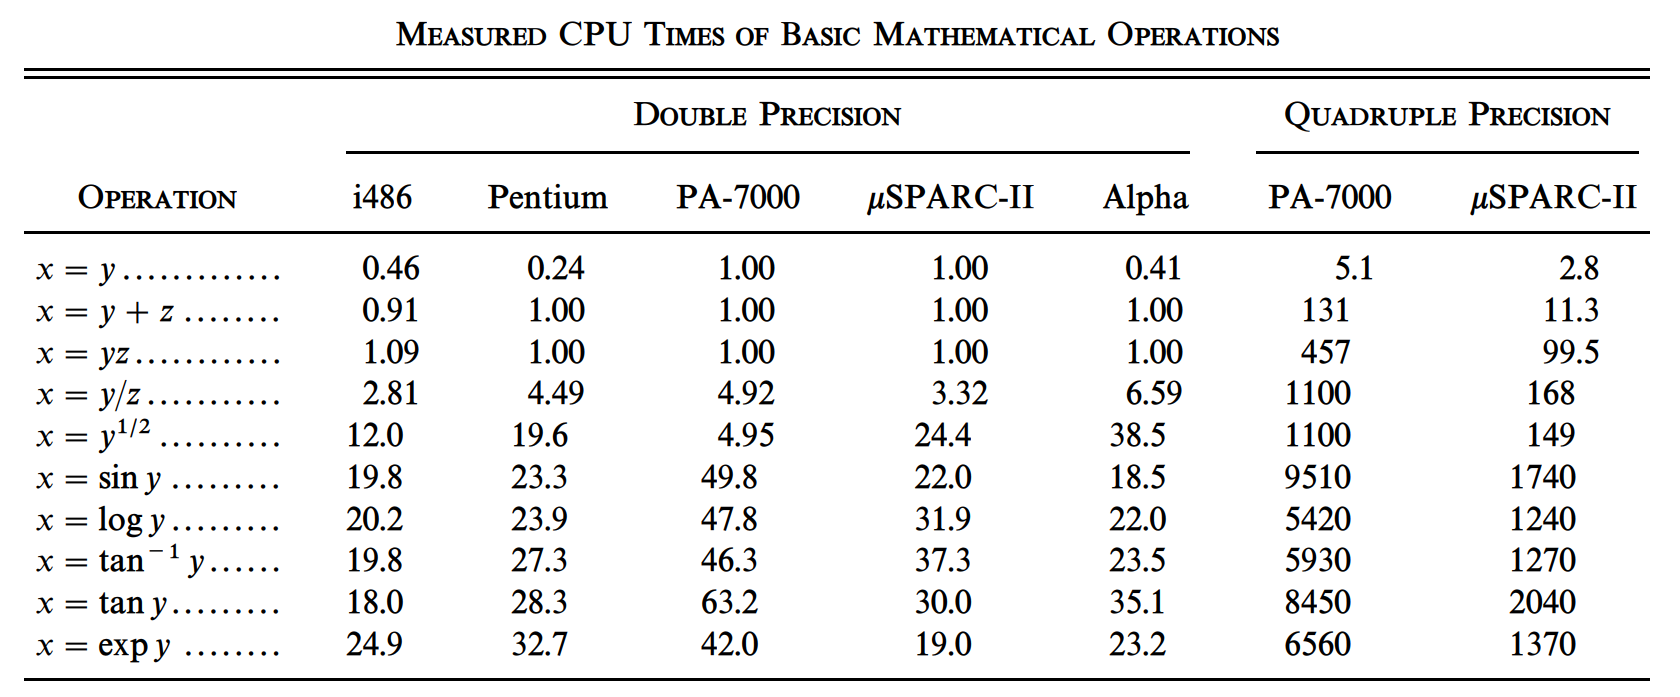
\includegraphics[width=.95\textwidth]{../../../figures/cpu_instruction_speed.png}
    \vspace{20pt}
    \caption{Amount of clock cycle for mathematical operations in various processors \cite{cpu_instruction_speed}.}
\end{figure}

\subsection{Concurrency}

Concurrency in programming refers to the ability of a program to execute multiple tasks or processes simultaneously. It allows different parts of a program to make progress independently, potentially improving performance, responsiveness, and resource utilization.

Concurrency in single core can be achieved by implementing clever scheduling of list of operations called \textit{threads}. This results in non-blocking execution of multiple threads, but only one thread would be executed at any given time. 
True concurrency on the other hand, can only be achieved by using multiple cores. Each core would be able to execute one thread at any time.

Programs that implement concurrency using multiple cores executes more operations per clock cycle. 
However, this does not directly lead to an improved performance due to the heavy burden of scheduling and managing multiple threads.

Threads utilize \textit{mutexes}, short for "mutual exclusion," 
to synchronize and manage access to shared resources 
in a multi-threaded or multi-process environment. 

\subsection{Object Oriented Programming}

Object-Oriented Programming (OOP) is a programming paradigm that revolves around the concept of objects. 
Definition called class serves as a blueprint that defines the structure and behavior of objects. 
Each object encapsulates both data, and the functions that manipulate that data. 
This encapsulation promotes modular code design and enhances data security by controlling access to the object's internal state. 

In OOP, \textit{inheritance} enables the creation of new classes based on existing ones, facilitating code reuse and hierarchy. 
\textit{Polymorphism} allows objects of different classes to be treated uniformly through a common interface, enhancing flexibility and extensibility. 
By providing abstraction, OOP simplifies complex systems by focusing on essential features and interactions, making software development more manageable, scalable, and maintainable.

%%%%%%

\begin{thebibliography}{9}
    \bibitem{cpu_instruction_speed}
    Fukushima, Toshio. (2001). \emph{Reduction of Round-off Errors in Symplectic Integrators}. The Astronomical Journal. 121. 1768-1775. 
\end{thebibliography}

\end{document}